\documentclass{standalone}
\usepackage{tikz}

\begin{document}
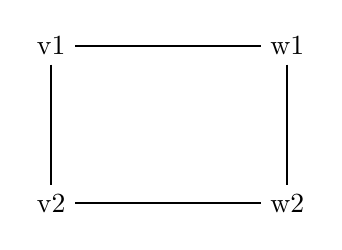
\begin{tikzpicture}[node distance=2cm]

% Nodes for C1
\node (v1) at (0,0) {v1};
\node (v2) at (0,-2) {v2};

% Nodes for C2
\node (w1) at (3,0) {w1};
\node (w2) at (3,-2) {w2};

% Solid arcs within C1 and C2
\draw[thick] (v1) -- (v2);
\draw[thick] (w1) -- (w2);

% Solid arcs between C1 and C2
\draw[thick] (w1) -- (v1);
\draw[thick] (w2) -- (v2);

% Dashed arcs between C1 and C2
\draw[dashed] (v1) -- (w1);
\draw[dashed] (v2) -- (w2);

\end{tikzpicture}
\end{document}